\section{Rigidez}

La rigidez es un fenómeno que asociamos a un problema de valor inicial.
Más que una característica matemática,
que podría ser definida de forma precisa,
es un conjunto de complicaciones que surgen
en la resolución de ciertos problemas.

\subsection{Un primer problema rígido}

Consideremos el problema de valor inicial
\begin{equation}\label{prb:rigid1}
    \begin{cases}
        y'(t) = 5\nume^{5t}(y-t)^2 + 1 \\
        y(0)
    \end{cases}
    \qq{para $t$ en $[0,1]$ o $[0,8]$}
\end{equation}
cuya solución analítica es $y(t) = t - \nume^{-5t}$.
Si intentamos resolverlo con el método de RK4
podemos construir la \cref{tab:rigid-problem-rk4-step-error-comparison}.
Observamos un fenómeno extraño.
Si el paso es menor que $0.2419$
el método obtiene unas cotas de error razonables
que se van reduciendo conforme disminuímos el tamaño del paso.
Sin embargo, si el paso es mayor o igual que $0.2419$,
el error del método se dispara.

\begin{table}[h]
    \centering
    \begin{tabular}{lll}
        \textbf{Tam. paso} & \textbf{Error Abs.} & \textbf{Error Rel.} \\
        \hline \\
        0.2001 & 0.0192308 & 0.00123008 \\
        0.2101 & 0.0463702 & 0.00266692 \\
        0.2201 & 0.0914377 & 0.00529422 \\
        0.2301 & 0.163178  & 0.0101477 \\
        0.2411 & 0.287569  & 0.0215778 \\
        0.2413 & 0.290396  & 0.0220027 \\
        0.2415 & 0.293245  & 0.0224769 \\
        0.2417 & 0.296118  & 0.0230281 \\
        0.2419 & inf       & inf \\
        0.2421 & inf       & inf \\
        0.2423 & inf       & inf
    \end{tabular}
    \caption{Error del método de RK4 para resolver el \cref{prb:rigid1}}
    \label{tab:rigid-problem-rk4-step-error-comparison}
\end{table}

Cuando integramos una ecuación diferencial cuyas derivadas tenemos acotadas,
la intuición\footnote{
    Justificada por las fórmulas de error que hemos obtenido,
    ya que una aproximación del error es $C\vy^{(p)}(\xi)h^p$.
}
nos dice que el tamaño del paso
podría ser grande en zonas donde la variación de la curva es pequeña
y debería ser más pequeño en intervalos donde la variación es grande.
También asumimos que podemos controlar el error
eligiendo un tamaño de paso adecuado u
obtener una aproximación del mismo
comparando una solución con otra donde hemos reducido el tamaño del paso.
Sin embargo, en el problema anterior vemos que el error,
si el paso no es más pequeño que un umbral\footnote{
    Podemos probar con otros métodos de paso fijo.
    Veremos que el umbral cambia en función del método.
},
se dispara.
Y por tanto la solución que estamos calculando
no converge paulatinamente hasta ese valor.

\subsection{Definición}

La característica que hemos visto no es atribuíble a la solución
$y(t) = t - \nume^{-5t}$,
puesto que podemos cambiar el problema para que siga teniendo la misma solución
y no se dispare el error.
Por tanto, la rigidez es una característica de un problema de valor inicial,
y no de una solución a ese problema.

Aparte del fenómeno anterior,
hay otros que habitualmente se atribuyen a los problemas que llamamos rígidos.
Enumeramos tres.
\begin{enumerate}
    \item Si el paso no está por debajo de un umbral,
    el error se dispara.
    \item Si utilizamos un método de paso adaptativo para resolver el problema,
    el método acaba porque sobreestima el error y determina que
    el paso que necesitaría utilizar sería menor que el mínimo permitido.
    Es un fenómeno que también se da en el problema anterior,
    pero si comparamos con la solución analítica vemos que en realidad
    el error del método cumple la tolerancia pedida.
    \item Si utilizamos un método de paso fijo tradicional,
    obtenemos una solución que oscila alrededor de la solución analítica.
    Por tanto, aunque la aproxime bien lo hace con un comportamiento diferente.
\end{enumerate}

Querríamos dar una definición precisa de problema rígido
basada en estos fenómenos.
Sin embargo, para cualquiera de ellos, podemos encontrar problemas
que nuestra definición tiene que considerar rígidos porque
presentan el resto de los fenómenos
pero que excluirían ese.
Lo que sí podemos es reconocer características que son comunes
a los problemas que presenten estos fenómenos.

Por ejemplo,
un sistema lineal de coeficientes constantes podría definirse como rígido
cuando todos sus valores propios, $\lambda_1,\ldots,\lambda_n$,
tienen parte real negativa y el coeficiente
\begin{equation*}
    \frac{\abs{\Re\lambda_M}}{\abs{\Re\lambda_m}}
    \qq{siendo $M$ y $m$ tales que
    $\abs{\Re\lambda_M} \ge \abs{\Re\lambda_k} \ge \abs{\Re\lambda_m}$
    para todo $1 \le k \le n$.}
\end{equation*}
es ``grande''.

De ahora en adelante utilizaremos la definición dada en clase,
que se basa en la idea de que los problemas rígidos sean aquellos
para los que no podamos asegurar que el error relativo sea pequeño.

\begin{definition}
    Dado un problema de valor inicial con derivada $\vy$
    que proporcione una estimación del error de la forma
    \begin{equation*}
        C\vy^{(p)}(\xi)h^p
    \end{equation*}
    donde $C$ y $p$ son constantes que dependen del método,
    $h$ el tamaño del paso y $\xi$ un punto del intervalo solución,
    diremos que estamos antes un \emph{problema rígido} si
    $\vy^{(p)}(\xi)$ crece de forma no acotada
    y en mayor proporción que $\vy(t)$.
\end{definition}

\subsection{Tamaño de paso umbral}

Siguiendo la definición de problema rígido,
un ejemplo de solución que tiende a cero rápidamente
pero cuyas derivadas no tanto es
$y(t) = \nume^{\lambda t}$ con $\lambda < 0$.
$y^{(p)} = \lambda^p\nume^{\lambda t}$.
El lector encontrará sencillo
escribir una ecuación diferencial con esa solución\footnote{
    Cuanto más grande sea el valor de $\lambda$ mejor será el ejemplo.
    Don Francisco sugiere que $\lambda$ debería ser grande.
    Pone como ejemplo $-30$.
}.

Para este problema concreto,
podemos estudiar cómo se comportan los métodos que conocemos.

\subsubsection{Método de Euler}

Para el método de Euler tendríamos una sucesión de la forma
\begin{equation*}
    \begin{cases}
        w_{i+1} = w_i + hf(t_i, w_i) = (1 + h\lambda)w_i \\
        w_0 = \alpha
    \end{cases}
\end{equation*}
de manera que $w_n = (1 + h\lambda)^w_0$,
mientras que la solución $y(t_n) = \nume^{\lambda t_n} = \nume^{n\lambda h}$.

Si queremos que el método de Euler se comporte como la solución analítica,
$w_n$ debería tender a $0$,
pero eso solo pasará si $\abs{1 + h\lambda} < 1$.
El lector sabrá que eso equivale a que $h < \frac{2}{\abs{\lambda}}$.

También podemos llegar a la misma conclusión
sin conocer el comportamiento de la solución analítica.
Si suponemos que hay un error de redondeo en el valor inicial,
de forma que iniciamos el método con $w_0 = \alpha + \epsilon$,
entonces el error de aproximación del $w_n$ teórico del método sería
$\epsilon_n = (1 + h\lambda)^n\epsilon$.
Por tanto, también obtendríamos el límite $h < \frac{2}{\abs{\lambda}}$
si quisiésemos que el error no creciese de manera exponencial.

\subsubsection{Otros métodos de paso fijo}

Visto el ejemplo del método de Euler,
podemos plantearnos repetirlo con otros métodos de paso fijo.
En ese caso dado un método obtendríamos
\begin{equation}\label{eqn:polq-one-step}
    w_{i+1} = Q(h\lambda)w_i
\end{equation}
en función de un polinomio $Q(x)$,
y querríamos que $\abs{Q(h\lambda} < 1$.
Por ejemplo, para el método de Taylor de orden $n$ se tendría que
$Q(x) = 1 + x + \frac{x^2}{2} + \cdots + \frac{x^n}{n}$.
Y en general, obtener el umbral para $h$ sería más laborioso.

\subsubsection{Métodos multipaso}

Para un método multipaso general, tendríamos
\begin{equation*}
    \begin{cases}
        w_i =
        a_0w_{i-m} + \cdots + a_{m-1}w_{i-1} + h\qty[
            b_0f(t_{i-m}, w_{i-m}) + \cdots + b_mf(t_i, w_i)
        ] \\
        w_0 = \alpha
    \end{cases}.
\end{equation*}
Aplicado al problema de prueba tendríamos que considerarlo como
una sucesión de recurrencia
\begin{equation*}
    (1 - h\lambda b_m)w_i
    - (a_{m-1} - h\lambda b_{m-1})w_{i-1}
    - \cdots
    - (a_0 + h\lambda b_0)w_{i-m} = 0,
\end{equation*}
cuyo polinomio característico sería
\begin{equation}\label{eqn:polq-multi-step}
    Q(z, h\lambda) =
    (1 - h\lambda b_m)z^m
    - (a_{m-1} - h\lambda b_{m-1})z^{m-1}
    - \cdots
    - (a_0 - h\lambda b_0).
\end{equation}

Si conocemos $w_0,\ldots,w_{n-1}$
y las raíces $\beta_1,\ldots,\beta_m$ de $Q(x, y)$
y son todas diferentes %TODO esto de qué teorema señores? DE QUÉ TEOREMA?
entonces las soluciones a esa sucesión serían de la forma
\begin{equation*}
    w_n = \sum_{i=1}^m C_i\beta_i^n,
\end{equation*}
para una constantes $C_1,\ldots,C_n$
que dependerían también de la condición inicial,
y tenderían a $0$ si $\abs{\beta_k} < 1$ para todo $1 \le k \le m$.

\subsection{A-Estabilidad}

En nuestro intento por caracterizar
qué métodos son mejores para resolver problemas rígidos,
vamos a tomar como referencia el problema de valor inicial
%TODO por qué tomamos k en C de repente?
$y' = ky$, $y(0) = 1$ para $k \in \C$
que hemos trabajado en la sección anterior
para analizar el comportamiento de diferentes métodos
ante problemas rígidos.

\begin{definition}
    Dado un método numérico a un paso, se define
    la \emph{Región de estabilidad absoluta} $R$
    como
    \begin{equation*}
        R = \qty{h\lambda \in \C : \abs{Q(h\lambda)} < 1},
    \end{equation*}
    donde $Q(x)$ es el polinomio que aparece en \eqref{eqn:polq-one-step}.

    Para un método numérico multipaso, se define como
    \begin{equation*}
        R = \qty{h\lambda \in \C :
        \text{$\abs{\beta_i} < 1$ para todas las raíces de $Q(z, h\lambda)$}},
    \end{equation*}
    donde $Q(z, h\lambda)$ es el polinomio que aparece en
    \eqref{eqn:polq-multi-step}.
\end{definition}

\begin{remark}
    La definición anterior determina una región donde
    debe encontrarse $h\lambda$ para evitar los problemas de estabilidad.
    Nos gustaría tener métodos
    cuya región de estabilidad fuese tan grande como sea posible.
\end{remark}

\begin{definition}
    Un método se dice $A$-estable si su región de estabilidad
    contiene el semiplano izquierdo.
\end{definition}

\begin{figure}[p]
    \centering
    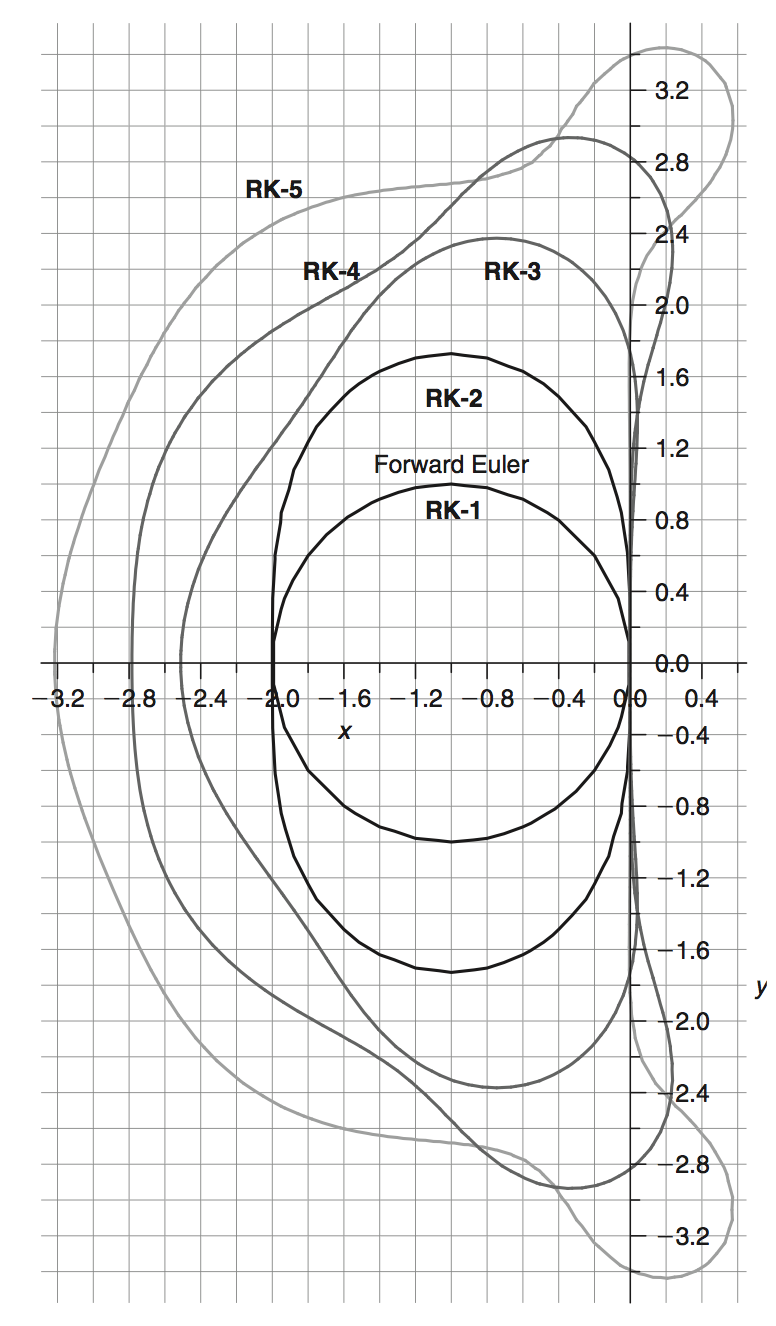
\includegraphics{media/RK-A-stability-regions.png}
    \caption{Región de estabilidad de los métodos de Runge-Kutta}
\end{figure}

%TODO Esto habrá que ponerlo más tarde:
% figureas para los métodos adams, adams-implícitos y adams-bashforth (PECE)

% Iserles pág 60
\begin{theorem}
    Ningún método explícito de Runge-Kutta puede ser $A$-estable.
\end{theorem}

% \begin{remark}
%     En realidad no hemos definido lo que es
%     un método explícito de Runge-Kutta todavía.
%     La definición que hemos dado de método de Runge-Kutta
%     se corresponde con los métodos explícitos.
%     A continuación estudiaremos los métodos implícitos.
% \end{remark}

% Iserles pág 67
\begin{theorem}
    El mayor orden de un método multipaso $A$-estable es $2$.
\end{theorem}

A continuación veremos como los métodos implícitos son en general
mejores para los problemas rígidos.

\section{Métodos Implícitos}

Los métodos implícitos son aquellos que
necesitan resolver una ecuación en la que la incógnita
es el siguiente punto de una solución.

\subsection{Método de Euler implícito o hacia atrás}

\begin{method}{Método de Euler hacia atrás}
    El \emph{método de Euler hacia atrás} determina,
    dado el problema \ref{eqn:pvi} y un paso $h > 0$:
    \begin{equation}\label{eqn:backwardseulersol}
    \begin{cases}
        w_0 = y_0 \\
        w_{i+1} = w_i + h\cdot f(t_{i+1}, w_{i+1}), \forall i=0,\dots, n-1
    \end{cases}
    \end{equation}
    Siendo $t_i = t_0 + i\cdot h$ para $i \in \qty{0,\ldots, n}$.
\end{method}

%TODO el método de euler es estable

\begin{proposition}
    El método de Euler hacia atrás es consistente.
\end{proposition}

\begin{proof}
    A partir de \eqref{eqn:backwardseulersol}, tenemos que 
    \begin{equation*}
        y(t + h) - y(t) - hf(t+h, y(t+h)) =
        hy'(t + h) + \frac{h^2}{2}y''(\xi) - hy'(t+h) =
        \frac{h^2}{2}y''(\xi).
    \end{equation*}
    Y por tanto, si $\norm{y''}$ está acotada (en el intervalo de resolución),
    $\lim_{h \to 0} \frac{Z(h)}{h} = 0$.
\end{proof}

% \begin{remark}
%     Como el método es consistente es también convergente
% \end{remark}

\begin{proposition}
    El método de Euler hacia atrás es $A$-estable.
\end{proposition}

\begin{proof}
    Fijado el problema $y' = y$, escribimos
    \begin{equation*}
        w_{i+1} = w_i + hf(t_{i+1}, w_{i+1}) = w_i + h\lambda w_{i+1}.
    \end{equation*}
    Reescribiendolo en forma de euación de recurrencia
    llegaríamos a estudiar el polinomio
    \begin{equation*}
        (1 - h\lambda)z - 1 = 0,
    \end{equation*}
    cuya única raíz es $z = \frac{1}{1 - (h\lambda)}$.
    Como
    \begin{equation*}
        \norm{\frac{1}{1 - (h\lambda)}} < 1 \iff
        \norm{1 - (h\lambda)} > 1,
    \end{equation*}
    la región de estabilidad son todos los puntos $(h\lambda) \in \C$
    a distancia mayor que $1$ de $1 \in \C$,
    lo cual incluye todo el semiplano izquierdo.
\end{proof}

\subsection{Método del trapecio}

\begin{method}{Método del Trapecio}
    El \emph{método del trapecio} determina,
    dado el problema \ref{eqn:pvi} y un paso $h > 0$:
    \begin{equation}\label{eqn:trapezoidalsol}
    \begin{cases}
        w_0 = y_0 \\
        w_{i+1} = w_i + \frac{h}{2}\qty(
            f(t_i, w_i) + f(t_{i+1}, w_{i+1})
        ), \forall i=0,\dots, n-1
    \end{cases}
    \end{equation}
    Siendo $t_i = t_0 + i\cdot h$ para $i \in \qty{0,\ldots, n}$.
\end{method}

\begin{proposition}
    El método del trapecio hacia atrás es un método consistente de orden $2$.
\end{proposition}

\begin{proof}
    A partir de \eqref{eqn:trapezoidalsol}, tenemos que 
    \begin{multline*}
        y(t+h) - y(t) - \frac{h}{2}\qty\bigg(f(t, y(t)) + f(t+h, y(t+h))) = \\
        hy'(t) + \frac{h^2}{2}y''(t) + \frac{h^3}{6}y'''(\xi)
        - \frac{h}{2}\qty\bigg(y'(t) - y'(t+h)) = \\
        hy'(t) + \frac{h^2}{2}y''(t) + \frac{h^3}{6}y'''(\xi)
        - \frac{h}{2}\qty\bigg(2y'(t) + hy''(t) + \frac{h^2}{2}y'''(\xi_2)) = \\
        \frac{h^3}{6}\qty\bigg(y'''(\xi_1) - y'''(\xi_2)).
    \end{multline*}
    Y por tanto, si $\norm{y'''}$ está acotada (en el intervalo de resolución),
    $\norm{\frac{Z(h)}{h}} \le ch^2\max{\norm{y'''}}$
    para una constante $c$,
    y el método es consistente y de orden $2$.
\end{proof}

\begin{proposition}
    El método del trapecio es $A$-estable.
\end{proposition}

\begin{proof}
    Tomando los coeficientes de la ecuación del método,
    \begin{equation*}
        w_{i+1} = w_i + \frac{1}{2}hf(t_i, w_i) + \frac{1}{2}f(t_{i+1}, w_{i+1}),
    \end{equation*}
    obtenemos el polinomio
    $Q(z, h\lambda) = \qty(1 - \frac{h\lambda}{2})z - \qty(1 + \frac{h\lambda}{2})$
    cuya única raíz es
    \begin{equation*}
        z = \frac{1 + \frac{h\lambda}{2}}{1 - \frac{h\lambda}{2}} =
        \frac{2 + h\lambda}{2 - h\lambda}.
    \end{equation*}

    Si tomamos $h\lambda = a + b\iunit$ con $a \le 0$, entonces
    \begin{equation*}
        \norm{\frac{2 + h\lambda}{2 - h\lambda}} =
        \frac{\norm{(2+a) + b\iunit}}{\norm{(2-a) + b\iunit}}
    \end{equation*}
    que es menor que $1$ porque $2 - a > 2 + a$.
    Por tanto, el método es $A$-estable.
\end{proof}

\subsection{Fórmulas de diferenciación hacia atrás}

Dado un método a $m$-pasos genérico
\begin{equation*}
    w_i = a_0w_{i-m} + \dots + a_{m-1}w_{i-1} + h\qty[
        b_0f(t_{i-m}, w_{i-m}) + \dots + b_{m-1}f(t_{i-1}, w_{i-1})
        + b_mf(t_i, w_i)
    ]
\end{equation*}
vamos a definir los polinomios
\begin{align*}
    \rho(z) = z^m -& a_{m-1}z^{m-1} + \dots - a_0 \qq{y} \\
    \sigma(z) = b_mz^m +& b_{m-1}z^{m-1} + \dots + b_0.
\end{align*}

\begin{definition}
    Un método a $m$-pasos es una fórmula de diferenciación (BDF) hacia atrás si
    \begin{itemize}
        \item el método es de orden $m$ y
        \item $\sigma(z) = \beta w^m$ con $\beta \ne 0$.
    \end{itemize}
\end{definition}

\begin{lemma}\label{lmm:bdf-parameters}
    Si un método es una BDF, entonces,
    siendo $\beta$ en las condiciones de la definición anterior,
    \begin{equation*}
        \beta = \qty(\sum_{i=1}^m \frac{1}{i})^{-1} \qq{y}
        \rho(z) = \beta\sum_{i=1}^m \frac{1}{j}z^{m-j}(z-1)^j.
    \end{equation*}
\end{lemma}

\begin{theorem}
    Una BDF de orden $m$ es estable y convergente si y solo si $1 \le m \le 6$.
\end{theorem}

\subsubsection{Fórmulas de diferenciación hacia atrás de orden 2 y 3}

Usaremos el \cref{lmm:bdf-parameters} para obtener los coeficientes.
Para orden $2$,
\begin{gather*}
    \beta = \qty(1 + \frac{1}{2})^{-1} = \frac{2}{3} \qq{y} \\
    \rho(z) = \frac{2}{3}\qty[z(z-1) + \frac{1}{2}(z-1)^2] =
    \frac{2}{3}\qty[\frac{3}{2}z^2 - 2z + \frac{1}{2}] =
    z^2 - \frac{4}{3} + \frac{1}{3}.
\end{gather*}
Lo que nos da proporciona el siguiente método.

\begin{method}{Fórmula de diferenciación hacia atrás de orden $2$}
    \begin{equation*}
        w_i = - \frac{1}{3}w_{i-2} + \frac{4}{3}w_{i-1}
            + \frac{2}{3}hf(t_i, w_i).
    \end{equation*}
\end{method}

Podemos repetir los cálculos para el orden $3$.

\begin{method}{Fórmula de diferenciación hacia atrás de orden $3$}
    \begin{equation*}
        w_i = \frac{2}{11}w_{i-3} - \frac{9}{11}w_{i-2} + \frac{18}{11}w_{i-1}
            + \frac{11}{6}hf(t_i, wi).
    \end{equation*}
\end{method}

\begin{remark}
    El método de Euler hacia atrás es la BDF de orden $1$.
\end{remark}

\begin{figure}[h]
    \centering
    \begin{subfigure}{0.3\textwidth}
        \centering
        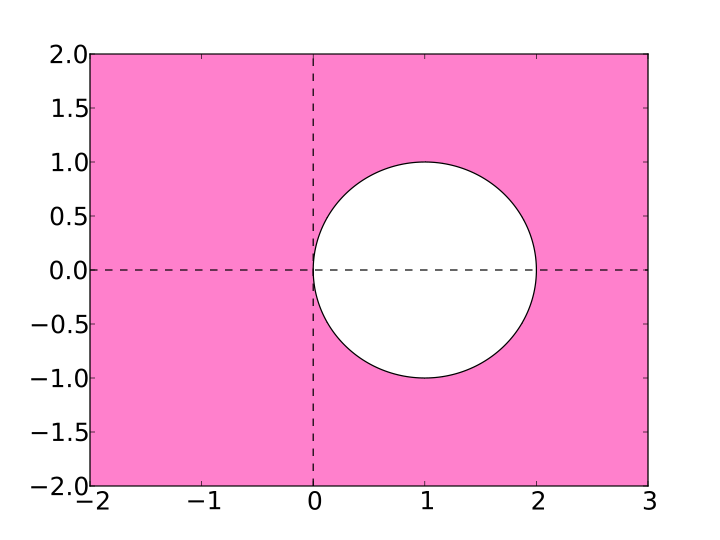
\includegraphics[width=\textwidth]{media/BDF1-A-stability-region.svg.png}
        \caption{BDF1}
    \end{subfigure}
    \begin{subfigure}{0.3\textwidth}
        \centering
        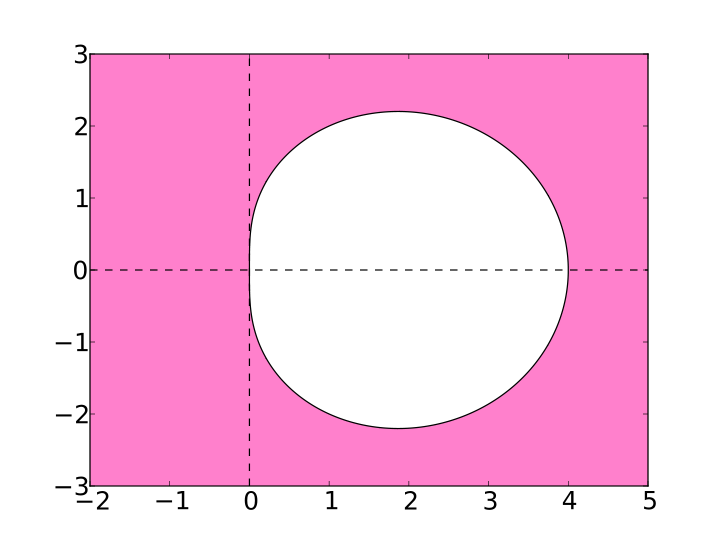
\includegraphics[width=\textwidth]{media/BDF2-A-stability-region.svg.png}
        \caption{BDF2}
    \end{subfigure}
    \begin{subfigure}{0.3\textwidth}
        \centering
        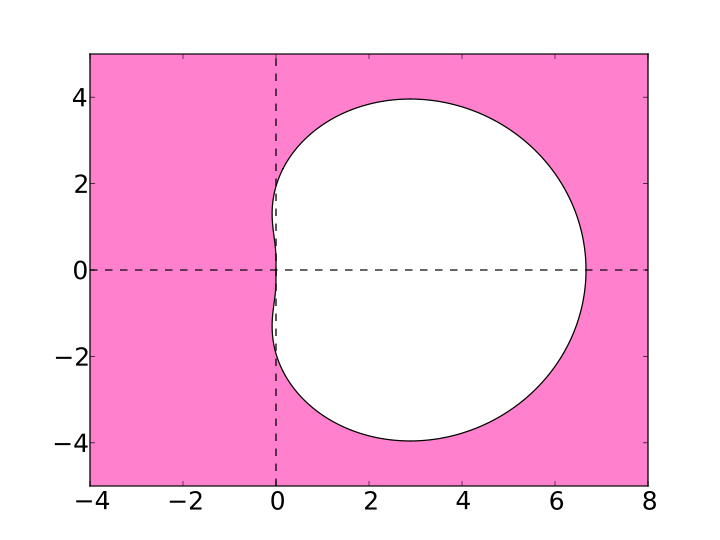
\includegraphics[width=\textwidth]{media/BDF3-A-stability-region.svg.png}
        \caption{BDF3}
    \end{subfigure}

    \begin{subfigure}{0.3\textwidth}
        \centering
        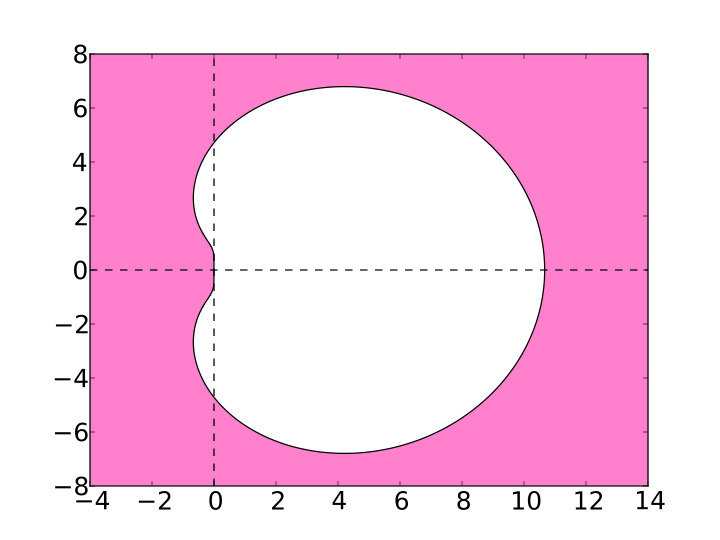
\includegraphics[width=\textwidth]{media/BDF4-A-stability-region.svg.png}
        \caption{BDF4}
    \end{subfigure}
    \begin{subfigure}{0.3\textwidth}
        \centering
        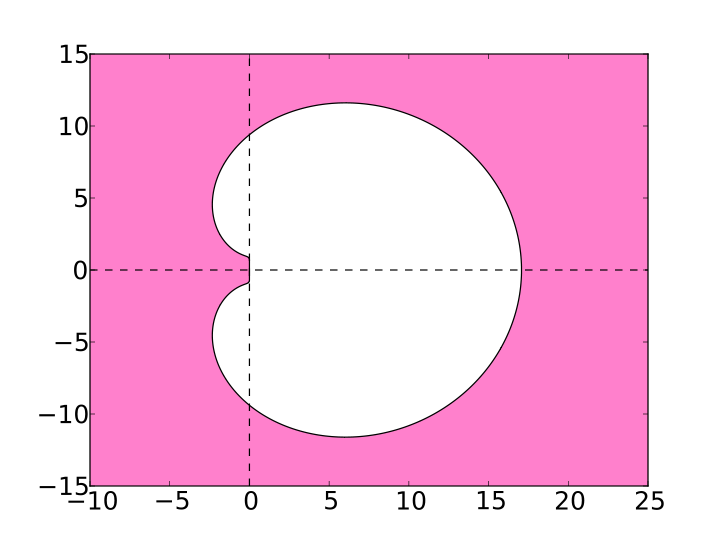
\includegraphics[width=\textwidth]{media/BDF5-A-stability-region.svg.png}
        \caption{BDF5}
    \end{subfigure}
    \begin{subfigure}{0.3\textwidth}
        \centering
        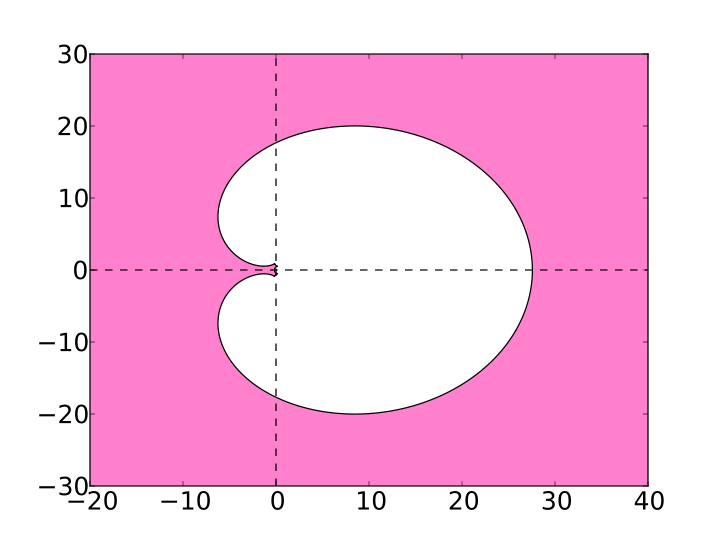
\includegraphics[width=\textwidth]{media/BDF6-A-stability-region.svg.png}
        \caption{BDF6}
    \end{subfigure}
    \caption{Región de convergencia para las $6$ BDF estables}
\end{figure}

%TODO hay que poner métodos de Runge-Kutta implícitos?
